\documentclass[10pt,landscape]{article}
\usepackage[italian]{babel}
\usepackage[T1]{fontenc}
\usepackage[utf8]{inputenc}
\usepackage{multicol}
\usepackage{multirow}
\usepackage{calc}
\usepackage{ifthen}
\usepackage[landscape]{geometry}
\usepackage{hyperref}
\usepackage{amsmath}
\usepackage{amssymb}
\usepackage{tabularx}
\usepackage{caption}
\usepackage{verbatim}
\usepackage{systeme}
\usepackage{nicefrac}
\usepackage{accents}
\usepackage{enumitem}
\usepackage[printwatermark]{xwatermark}
\usepackage{tikz}
\usetikzlibrary{calc,matrix,arrows,intersections,decorations.pathreplacing,shapes.misc}
\usepackage[compact]{titlesec}
\usepackage{microtype}
\usepackage[flushleft]{threeparttable}
\usepackage{textcomp}
\usepackage{pifont}
\usepackage{pgfplots}
\usepackage[arrowdel]{physics}
\usepackage{siunitx}
\usepackage{booktabs}
\usepackage{stmaryrd}
\usepackage{chemformula}
\usepackage{fancyhdr}
\usepackage{lastpage}

% Ranges of numbers
\sisetup{range-phrase=--}

% Page margins
\geometry{top=.5in,left=.5in,right=.5in,bottom=.5in,headsep=0in}

% Turn off header and footer
\pagestyle{empty}

% Reduce size of \section e \subsection
\titleformat{\section}{\normalfont\large\bfseries}{\thesection}{1em}{}
\titleformat{\subsection}{\normalfont\normalsize\bfseries}{\thesubsection}{1em}{}
\titleformat{\subsubsection}{\normalfont\small\bfseries}{\thesubsection}{1em}{}
\titlespacing{\section}{0pt}{0ex}{-0.5ex}
\titlespacing{\subsection}{0pt}{0ex}{-0.5ex}
\titlespacing{\subsubsection}{0pt}{0ex}{-0.5ex}

% Define BibTeX command
\def\BibTeX{{\rm B\kern-.05em{\sc i\kern-.025em b}\kern-.08em
		T\kern-.1667em\lower.7ex\hbox{E}\kern-.125emX}}

% Don't print section numbers
\setcounter{secnumdepth}{0}

\setlength{\parindent}{0pt}
\setlength{\parskip}{0pt plus 0.5ex}

\setlist[itemize]{noitemsep, nolistsep}

% No idea, without this tikz gives a warning
\pgfplotsset{compat=1.16}

\pgfmathdeclarefunction{gauss}{2}{%
  \pgfmathparse{1/(#2*sqrt(2*pi))*exp(-((x-#1)^2)/(2*#2^2))}%
}

\newcommand{\sla}{\shortleftarrow}
\newcommand{\sra}{\shortrightarrow}

\DeclareMathOperator{\Nus}{Nu}
\DeclareMathOperator{\Rey}{Re}
\DeclareMathOperator{\Pra}{Pr}
\DeclareMathOperator{\Gra}{Gr}
\DeclareMathOperator{\Pec}{Pe}
\DeclareMathOperator{\Ray}{Ra}

\newcommand{\gaussiana}[4]{
	\begin{axis}[
		hide axis,
		axis lines=left,
		xtick=\empty,
		ytick=\empty,
		every axis plot post/.append style={mark=none,domain=-1:1,samples=50,smooth},
		xmin=#1,
		xmax=#2,
		ymin=#3,
		ymax=#4,
		width=5cm
	]
		\addplot[black] {gauss(0,0.6)};
	\end{axis}
}

\pagenumbering{arabic}
\pagestyle{fancy}
\fancyhead[R]{Pagina \thepage{} di \pageref{LastPage}}
\fancyhead[L]{}
\fancyfoot[C]{}
\renewcommand{\headrulewidth}{0pt}

% section color
\usepackage{xcolor}
\usepackage{sectsty}
\definecolor{sectioncolor}{HTML}{FF0000}
\definecolor{subsectioncolor}{HTML}{580000}
\sectionfont{\color{sectioncolor}}
\subsectionfont{\color{subsectioncolor}}

% \color{white}
% \pagecolor{black}

\begin{document}

\raggedright
\footnotesize
\begin{multicols}{3}

% multicol parameters
% These lengths are set only within the two main columns
%\setlength{\columnseprule}{0.25pt}
\setlength{\premulticols}{1pt}
\setlength{\postmulticols}{1pt}
\setlength{\multicolsep}{1pt}
\setlength{\columnsep}{2pt}

{\Large{\textbf{Fisica Tecnica}}}

\section{Concetti base}
\subsection{Conversioni}
\begin{tabular}{lr}
    \toprule
    \SI{1}{atm} & \SI{101325}{Pa} \\
    \SI{1}{ata} & \SI{98066,5}{Pa} \\
    \SI{1}{bar} & \SI{100000}{Pa} \\
    \SI{1}{psi} & \SI{6895}{Pa} \\ \midrule
    \SI{1}{kcal} & \SI{4186}{J} \\ \midrule
    $x\;\si{\degree C}$ & $x + \SI{273,15}{K}$ \\
    $x\;\si{\degree F}$ & $\frac{5}{9}(x + 459.67) \si{K}$ \\
    \bottomrule
\end{tabular}

\subsection{Costanti}
\begin{tabular}{ll}
    \toprule
    Costante dei gas ideali & $R=\SI{8314}{J/k mol.K}$ \\
    Entalpia solidif. \ch{H2O} & $h_{lst,\ch{H2O}} = \SI{-333}{kJ/kg}$ \\
    Entalpia evaporazione \ch{H2O} & $h_{lvt,\ch{H2O}} = \SI{2501.6}{kJ/kg}$ \\
    Entalpia sublimazione \ch{H2O} & $h_{svt,\ch{H2O}} = \SI{2834.6}{kJ/kg}$ \\
    Pressione punto triplo \ch{H2O} & $P_0 = \SI{611.2}{Pa}$ \\
    Temperatura punto triplo \ch{H2O} & $T_0 = \SI{0.01}{\degree C} = \SI{273.16}{K}$ \\
    Pressione stato critico \ch{H2O} & $P_{cr} = \SI{22.09}{MPa}$ \\
    Temperatura stato critico \ch{H2O} & $T_{cr} = \SI{647.3}{K}$ \\
    Calore specifico ghiaccio & $c_s = \SI{2093}{J/kg.K}$ \\
    Volume specifico ghiaccio & $v_s = \SI{0.00109}{m^3/kg}$ \\
    Calore specifico acqua & $c_s = \SI{4186}{J/kg.K}$ \\
    Volume specifico acqua & $v_s = \SI{0.001}{m^3/kg}$ \\
    Calore specifico medio vapore & $c_p = \SI{2009}{J/kg.K}$ \\
    \bottomrule
\end{tabular}

Masse atomiche (\si{kg/k mol}):
\[ \ch{H} = \si{1,008} \quad \ch{He} = \si{4,003} \quad \ch{C} = \si{12,011} \quad \ch{N} = \si{14,007} \]
\[ \ch{O} = \si{15,999} \quad \ch{Ne} = \si{20,18} \quad \ch{Ar} = \si{39,95} \quad \ch{Kr} = \si{83,798} \]

Masse molecolari:
\[ \ch{H2O} = \si{18,015} \quad \text{aria}(79/21) = 28,85 \quad \ch{CH4} = \si{16,043} \]

\subsection{Sistema termodinamico}
\begin{tabular}{lccc}
    \toprule
    & Calore & Lavoro & Massa\\ \midrule
    Adiabatico & no & & \\
    Diatermano & sì & & \\
    Rigido & & no & \\
    Deformabile & & sì & \\
    Chiuso (impermeabile) & & & no \\
    Aperto (permeabile) & & & sì \\
    Isolato & no & no & no \\
    \bottomrule
\end{tabular}

\subsection{Grandezze}
\begin{itemize}
    \item \textbf{Intensive}: non dipendono dall'estensione del sistema (temperatura, pressione, densità);
    \item \textbf{Estensive}: dipendono dall'estensione del sistema (massa, volume);
    \item \textbf{Estensive specifiche}: estensiva/estensiva ($v = \frac{V}{M}$).
\end{itemize}

\subsection{Legge di Duhem}
In un sistema semplice monocomponente il numero di parametri intensivi o estensivi specifici
necessari per descriverlo all'equilibrio è 2.


\subsection{Regola di Gibbs}
\[V = C + 2 - F\]

\begin{tabular}{ll}
    $V$ & numero di variabili intensive indipendenti \\
    $C$ & numero di componenti \\
    $F$ & numero di fasi \\
\end{tabular}

Ne deriva l'esistena di una legge di stato:
\[f(P, v, T) = 0\]

\subsection{Trasformazioni termodinamiche}
\begin{tabular}{p{3.1cm}p{4cm}}
    \toprule
    Trasformazione & Caratteristiche \\
    \midrule
    Quasi-statica o \newline internamente reversibile & Costituita da una successione di stati di equilibrio; può non essere reversibile \\
    Reversibile & Se percorsa in senso inverso, riporta sistema e ambiente nello stato iniziale \\
    Irreversibile & Non è rappresentabile su un diagramma di stato \\
    Chiusa o ciclica & Gli estremi della trasformazione coincidono \\
    Elementare & Se una delle grandezze di stato si mantiene costante durante la trasformazione \\
    \bottomrule
\end{tabular}

\subsection{Gas ideali}
Un gas può essere considerato ideale per pressioni minori di $\si{10\bar}$.

\[PV = nRT = MR^*T\]
\[Pv = R^*T \]
\begin{tabular}{ll}
    $P$ & pressione $[\si{\pascal}]$ \\
    $V$ & volume $[\si{m^3}]$ \\
    $n$ & numero di moli $[\si{\mol}]$ \\
    $R$ & costante universale dei gas ideali $\SI{8314}{\J/k\mol.\K}$ \\
    $R^*$ & costante del gas $R/Mm \; [\si{J/Kg.K}]$ \\
    $T$ & temperatura $[\si{\K}]$ \\
    $M_m$ & massa molecolare \\
\end{tabular}

\subsection{Gas reali}
Equazione di van der Waals:
\[\left(P + \frac{a}{v_m^2}\right)(v_m-b) = RT\]

\subsection{Liquidi e solidi}
\begin{align*}
    \dd{v} &= \left(\pdv{v}{T}\right)_P \dd{T} + \left(\pdv{v}{P}\right)_T \dd{P} \\
    \dd{v} &= \beta v \dd{T} - K_T v \dd{P}
\end{align*}

\begin{align*}
    \beta = \frac{1}{v} \left(\pdv{v}{T}\right)_P & \quad \text{coeff. di dilatazione termica isobaro} \\
    K_T = -\frac{1}{v} \left(\pdv{v}{P}\right)_T & \quad \text{coeff. di dilatazione termica isotermo} \\
\end{align*}

\section{Principi della termodinamica}

\subsection{Principi di conservazione}
\begin{itemize}
    \item Conserazione della \textbf{massa};
    \item Conserazione della \textbf{energia} (I principio);
    \item Conserazione della \textbf{entropia} (II principio);
\end{itemize}

\subsection{Primo principio della termodinamica per sistemi chiusi}
Per un sistema semplice all’equilibrio è definita una proprietà intrinseca (funzione di stato) detta energia interna $U$ la cui variazione è il risultato di interazioni del sistema con l’ambiente esterno.

L'energia che è immagazinata in un sistema e che non va a cambiare né l'energia cinetica del centro di massa, né quella potenziale (e neanche l'energia elastica o chimica o elettrica) è chiamata energia interna.

\[\Delta U = Q^\sla - L^\sra \]

\begin{tabular}{ll}
    $U$ & energia interna del sistema \\
    $Q^\sla$ & calore entrante nel sistema\\
    $L^\sra$ & lavoro uscente dal sistema\\
\end{tabular}

L'energia interna è una grandezza estensiva (additiva):
\[U_z = U_1 + U_2 + \ldots\]

Per una trasformazione ciclica:
\[\Delta U_{\text{ciclo}} = 0 \]

Per un sistema isolato:
\[\Delta U_{\text{isolato}} = 0\]

Primo principio in forma differenziale:
\[\dd{u} = \var{q^\sla} - \var{l^\sra}\]

\subsection{Secondo principio della termodinamica per sistemi chiusi}

Per un sistema all'equilibrio esiste una funzione di stato detta \textbf{entropia} $S$ la cui variazione per una trasformazione \emph{reversibile} è data da:
\[\Delta S = \int \frac{\var{Q_{rev}^\sla}}{T}\]

L'entropia è una grandezza estensiva (additiva):
\[
    S_z = S_1 + S_2 + \ldots \qquad \Delta S_z = \Delta S_1 + \Delta S_2 + \ldots
\]

La variazione di entropia totale di un sistema isolato è sempre maggiore di zero e tende a zero con il tendere dei processi alla reversibilità:
\[
    \Delta S_{\text{isolato}} \geq 0
\]  

In un sistema chiuso il \textbf{bilancio entropico} è dato da:
\[
    \Delta S = S_Q^\sla + S_{irr} \qquad \text{$S_Q^\sla$ dovuta dallo scmabio di calore $Q$}
\]
\[
    S_{irr} \ge 0 \qquad \text{segno}~S_Q^\sla = \text{segno}~Q^\sla
\]
\section{Trasformazioni}

\subsection{Lavoro termodinamico}

\begin{align*}
    \delta L^\sra &= PA\dd{s} = P\dd{V} \\
    \delta l^\sra &= P\dd{v} \\
    l^\sra &= \int_i^f P\dd{v}
\end{align*}

Il lavoro dipende dal percorso: \textbf{non} è funzione di stato.

\subsection{Calori specifici}

\begin{align*}
    \text{Capacità termica} &\qquad C_x = \left(\frac{\delta Q^\sla}{\dd{T}}\right)_x \\
    \text{Calore specifico} &\qquad c_x = \frac{1}{M} \left(\frac{\delta Q^\sla}{\dd{T}}\right)_x
\end{align*}

\begin{align*}
    \text{A pressione cost.} &\qquad c_P = \frac{1}{M} \left(\frac{\delta Q^\sla}{\dd{T}}\right)_P = \left(\frac{\delta q^\sla}{\dd{T}}\right)_P \\
    \text{A volume cost.} &\qquad c_v = \frac{1}{M} \left(\frac{\delta Q^\sla}{\dd{T}}\right)_v = \left(\frac{\delta q^\sla}{\dd{T}}\right)_v
\end{align*}

Inoltre si ha che
\begin{align*}
    \text{A pressione cost.} &\qquad c_P = \qty(\pdv{h}{T})_P\\
    \text{A volume cost.} &\qquad c_v = \qty(\pdv{u}{T})_v
\end{align*}

\subsection{Entalpia}

L'entalpia è una funzione di stato.
\[ h = u + Pv \]
\[ \dd{h} = \dd{u} + v\dd{P} + P\dd{v} = \delta q^\sla + v\dd{P} \]
\[ \delta q^\sla = \dd{h} - v\dd{P} \]

\subsection{Calori specifici per i gas ideali}
Nei gas ideali, a seguito di evidenze sperimentali, si ha che $u = u(T)$, ovvero l'\textbf{energia interna dipende solo dalla temperatura}. Inoltre anche siccome $h = u + PV$ e $Pv = R^*T$, otteniamo che $h = h(T)$.
Quindi $c_V$ e $c_P$ sono dipendenti solo dalla temperatura e si ha che
\begin{align*}
    \text{A pressione cost.} &\qquad c_P = c_P(T) = \qty(\dv{h}{T})\\
    \text{A volume cost.} &\qquad c_V = c_V(T) = \qty(\dv{u}{T})
\end{align*}

\textbf{Relazione di Mayer}
\[ c_P = \dv{h}{T} = \frac{\dd{u} + \dd{\qty(Pv)}}{\dd{T}} = \qty(\dv{u}{T}) + \dv{R^*T}{T} = c_v + R^* \]

\subsection{Calori specifici per un gas perfetto}
Per i gas \textbf{perfetti} (gas ideali per variazioni di temperatura non troppo elevate) i calori specifici non dipendono neanche dalla temperatura:

{\renewcommand\arraystretch{1.4}
\begin{tabular}{lcc}
    \toprule
    & $c_v$ & $c_p$ \\ \midrule
    Gas Monoatomico & $\frac{3}{2}R^*$ & $\frac{5}{2}R^*$ \\
    Gas Biatomico o Poliatomico lineare & $\frac{5}{2}R^*$ & $\frac{7}{2}R^*$ \\
    Gas Poliatomico non lineare & $\frac{6}{2}R^*$ & $\frac{8}{2}R^*$ \\
    \bottomrule
\end{tabular}}

\begin{tabular}{ll}
    Monoatomico & \ch{He}, \ch{Ar}, $\ldots$ \\
    Linare & \ch{O2}, \ch{N2}, \ch{H2}, \ch{CO2}, $\ldots$ \\
    Non lineare & \ch{CH4}, \ch{H2O}, $\ldots$ \\
\end{tabular}

\subsection{Calori specifici per i liquidi}

Liquido incomprimibile ideale $C_v = C_P = c(T)$.

Liquido incomprimibile perfetto $C_v = C_P = \text{cost}$.

\subsection{Politropiche}
Trasformazione quasi statica per un sistema con un \textbf{gas ideale} dove $c_x = \text{cost}$.

Si definisce indice della politropica il temrine $n = \frac{c_x-c_P}{c_x-c_V}$

\[
    Pv^n = \text{cost} \quad Tv^{n-1} = \text{cost} \quad \frac{T^n}{P^{n-1}} = \text{cost} \quad PT^{\frac{n}{1-n}} = \text{cost}
\]

\begin{tabular}{lcc}
    \toprule
    Trasformazione & $c_x$ & $n = \frac{c_x-c_P}{c_x-c_V}$ \\
    \midrule
    Isoterma & $\pm\infty$ & 1 \\
    Isocora & $c_v$ & $\pm\infty$ \\
    Isobara & $c_P$ & 0 \\
    Adiabatica & 0 & $k = \frac{c_p}{c_v}$ \\
    \bottomrule
\end{tabular}

Per $n \ne 1$ (quindi non isoterma) l'integrale del lavoro diventa:
\begin{align*}
    l^\sra = \int_1^2 P\dd{v} &= \frac{P_1v_1}{n-1} \qty[1-\qty(\frac{v_1}{v_2})^{n-1}] \\
    &= \frac{P_1v_1}{n-1} \qty[1-\qty(\frac{P_2}{P_1})^{\frac{n-1}{n}}]
\end{align*}
Per $n = 1$ (quindi isoterma) l'integrale del lavoro diventa:
\[ l^\sra = \int_1^2 P\dd{v} = P_1v_1\ln{\frac{v_2}{v_1}} = P_1v_1\ln{\frac{P_1}{P_2}} \]

\subsection{Diagramma T-s}

\begin{center}
    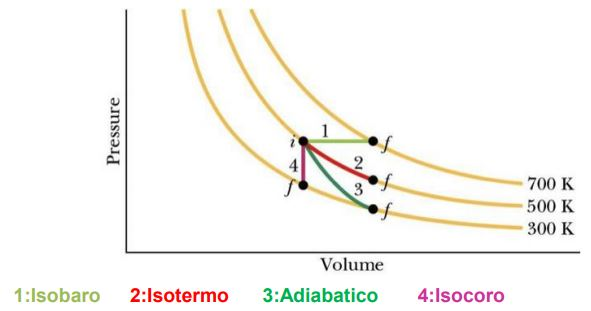
\includegraphics[height=3cm]{politropiche.JPG}
\end{center}

\begin{center}
    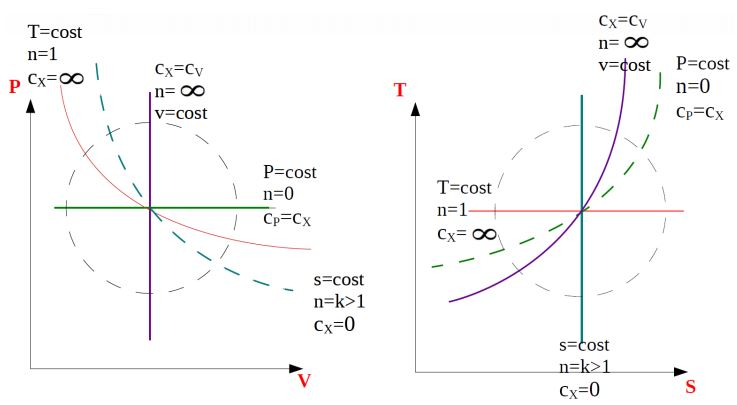
\includegraphics[height=3cm]{politropiche2.JPG}
\end{center}

L'area sottesa dalla curva in una trasformazione \emph{internamente reversibile} è uguale al calore scambiato dal sistema nella trasformazione:
\[ \dd{S}_{rev} = \frac{\dd{Q}_{rev}}{T} \qquad Q_{rev} = \int_i^f \dd{Q}_{rev} = \int_i^f T(S) \dd{S} \]

Nel piano T-s tutte le trasformazioni politropiche sono esponenziali:
\[T = T_0 e ^ { \frac{s-s_0}{c_x} }\]

\begin{tabular}{ll}
    Isoterme  (Isoentalpiche con gas ideali) & rette orizzontali \\
    Adiabatiche reversibili (isoentropiche) & rette verticale \\
    Isocore ($c_v < c_P$) & più ripide delle isobare \\
\end{tabular}

\section{SONO ARRIVATO A PAGINA 41}

\subsubsection{Per i gas perfetti}
\begin{tabular}{lll}
    \toprule
    Trasformazione & $l=\int P\dd{v}$ & $q = \int \dd{q}$ \\
    \midrule
    $P = \text{cost}$ & $P\Delta v$ & $c_p\Delta T$ \\
    $v = \text{cost}$ & 0 & $c_v\Delta T$ \\
    $T = \text{cost}$ & $R^*T\ln{\frac{v_2}{v_1}} =$ & $R^*T\ln{\frac{v_2}{v_1}} =$ \\
    & $-R^*T\ln{\frac{P_2}{P_1}}$ & $-R^*T\ln{\frac{P_2}{P_1}}$ \\
    $\dd{Q}=0$ & $-c_v\Delta T$ & 0 \\
    $c_x = \text{cost}$ & $(c_x-c_v)\Delta T$ & $c_x\Delta T$ \\
    \bottomrule
\end{tabular}

\subsubsection{Per i gas perfetti}
\[ \Delta u = c_v \Delta T \qquad \Delta h = c_p \Delta T \]
\begin{align*}
    \Delta s &= c_v \ln{\frac{T_2}{T_1}} + R^*\ln{\frac{v_2}{v_1}} \\
    &= c_p \ln{\frac{T_2}{T_1}} - R^*\ln{\frac{P_2}{P_1}} \\
    &= c_p \ln{\frac{v_2}{v_1}} + c_v\ln{\frac{P_2}{P_1}} \\
\end{align*}

\subsubsection{Per i liquidi incomprimibili}

Se perfetti:

\[ \Delta u = c \Delta T \qquad \Delta s = c \ln{\frac{T_2}{T_1}} \]

Se ideali $c_p = c(T)$, $\beta = 0$ e $K_T = 0$:
\[ \dd{h} = c(T)\dd{T} + v\dd{P} \qquad \dd{s} = c(T)\frac{\dd{T}}{T} \]

Se perfetti:
\[ \Delta h = c\Delta T + v \Delta P \]

\subsubsection{Miscelamenti}
In caso di miscelazione \textbf{adiabatica} di più gas:
\begin{itemize}
    \item Isobara: $\Delta H = 0$
    \item Isocora: $\Delta U = 0$
\end{itemize}

Legge di \textbf{Dalton}: il volume di una miscela di gas è uguale alla somma dei volumi che ognuno dei gas avrebbe se se fosse da solo nelle stesse condizioni di temperatura e pressione della miscela.

Legge di \textbf{Dalton}: la pressione di una miscela di gas è uguale alla somma delle pressioni che ognuno dei gas avrebbe se se fosse da solo nelle stesse condizioni di temperatura e volume della miscela.

\section{Macchina termodinamica}
La macchina termodinamica è un sistema termodinamico composto ed isolato che nel caso più semplice è realizzato da
\begin{itemize}
\item due serbatoi di calore
\item un serbatoio di lavoro
\item una macchina ciclica che è in grado di interagire con continuità con i serbatoi di calore e lavoro
\end{itemize}

\begin{description}
\item[Serbatoio di calore]
sistema termodinamico che scambia solo calore con l'esterno senza alterare il suo stato interno;
gli scambi avvengono con trasformazioni quasi-statiche internamente reversibili.
\item[Serbatoio di lavoro]
sistema termodinamico che scambia solo lavoro con l'esterno senza alterare il suo stato interno;
gli scambi avvengono con trasformazioni quasi-statiche internamente reversibili.
\end{description}

\subsubsection{Risoluzione problemi macchine termiche}
Bisogna impostare e risolvere il sistema contente le equazioni di bilancio
\[
    \begin{cases}
    \Delta U_Z = 0 \\
    \Delta S_Z = S_{irr} \\
    \end{cases} \qquad \begin{cases}
        \Delta U_C + \Delta U_F + \Delta U_{SL} + \Delta U_M = 0\\
        \Delta S_C + \Delta S_F + \Delta_{SL} + \Delta S_M = S_{irr}
    \end{cases}
\]

Per macchina motrice con masse infinite:
\[
    \begin{cases}
        -Q_C + Q_F + L = 0 \\
        -\frac{Q_C}{T_C} + \frac{Q_F}{T_F} = S_{irr} \\
    \end{cases}
\]

Per macchina operatrice con masse infinite:
\[
    \begin{cases}
        Q_C - Q_F - L = 0 \\
        \frac{Q_C}{T_C} - \frac{Q_F}{T_F} = S_{irr} \\
    \end{cases}
\]

\subsection{Rendimenti macchine termiche}
{\renewcommand{\arraystretch}{1.5}
\begin{tabular}{p{3.5cm}r}
\textbf{Macchina motrice} & $\eta = \frac{L}{Q_C} \quad \eta_{II} = \frac{\eta}{\eta_{rev}} = \frac{L}{L_{rev}} $ \\
→ serbatoi a massa infinita & $\eta = 1 - \frac{T_F}{T_C} - \frac{T_F}{Q_C}S_{irr}$ \\
\phantom{→}$\put(3,2){\line(0,1){5}}\to$ reversibile ($S_{irr} = 0$) & $\eta_{rev} = 1 - \frac{T_F}{T_C}$ \\
\\
\textbf{Macchina operatrice} & (serbatoi a temp. cost.) \\
→ frigorifera & $\varepsilon_f = \frac{Q_F}{L} \quad \eta_{II} = \frac{\varepsilon}{\varepsilon_{rev}} = \frac{L_{rev}}{L}$ \\
\phantom{→}$\put(3,2){\line(0,1){5}}\to$ reversibile & $\varepsilon_{f,rev} = \frac{T_F}{T_C - T_F}$ \\
→ pompa di calore & $\varepsilon_{pdc} = \frac{Q_C}{L}$ \\
\phantom{→}$\put(3,2){\line(0,1){5}}\to$ reversibile & $\varepsilon_{pdc,rev} = \frac{T_C}{T_C - T_F}$ \\
\end{tabular}
}

\section{Sistemi aperti}

\subsection{Bilancio di massa}
\[ \dv{m}{t} = \sum_i \dot{m}_i^\sla \]

\subsubsection{Equazione di continuità}
\[ \dot{m} = \rho w \Omega \]

\subsection{Bilancio di energia}
\[ \dv{E}{t} = \sum_i \dot{E}_i^\sla \]
dove $E$ rappresenta l'energia associata al trasporto di massa e al lavoro e calore scambiato

\subsubsection{Lavoro di pulsione}
\[ L_P^\sla = - \int^{V}_{V+V_m} P\dd{V} = PV_m = m_i P v_i \]
\subsubsection{Energia associata al trasporto di massa}
\[ E_m = \sum_i m_i^\sla \qty(u + gz + \frac{w^2}{2}) \]
\subsubsection{Bilancio energetico}
\[ \dv{E}{t} = \sum_i \dot{m}_i^\sla \qty(h + gz + \frac{w^2}{2}) + \dot{Q}^\sla - \dot{L_e}^\sra\]

\subsection{Bilancio di entropia}
\[ \dv{S}{t} = \sum_i \dot{m}_i^\sla s_i + \dot{S}_{Q^\sla} + \dot{S}_{irr} \]

\subsection{Regime stazionario}
\[ \dot{m}_{ingresso}^\sla = -\dot{m}_{uscita}^\sla \]

\[ \dot{m}^\sla\qty[(h_i - h_u) + g(z_i-z_u) + \frac{(w_i^2-w_u^2)}{2}] + \dot{Q}^\sla - \dot{L}_e^\sra = 0 \]

\[ \dot{m}^\sla (s_i - s_u) + \dot{S}_{Q^\sla} + \dot{S}_{irr} = 0 \]

\section{Macchina aperta}
\subsubsection{Turbina, compressore e pompa}
\[ \dot{m}^\sla (h_i - h_u) - \dot{L}_e^\sra = 0 \]
\[ \dot{m}^\sla (s_i - s_u) + \dot{S}_{irr} = 0 \]

\subsubsection{Scambiatore di calore}
\[ \dot{m}^\sla (h_i - h_u) + \dot{Q}^\sla = 0 \]
\[ \dot{m}^\sla (s_i - s_u) + \dot{S}_{Q^\sla} + \dot{S}_{irr} = 0 \]

\subsubsection{Diffusore (w↓) e ugello (w↑)}
\[  (h_i - h_u) + \frac{(w_i^2 - w_u^2)}{2} = 0 \]
\[ \dot{m}^\sla (s_i - s_u) + \dot{S}_{irr} = 0 \]

\subsubsection{Valvola di laminazione}
\[  (h_i - h_u) = 0 \]
\[ \dot{m}^\sla (s_i - s_u) + \dot{S}_{irr} = 0 \]

\subsection{Rendimento isoentropico}
\subsubsection{Turbina}
\[ \eta_{is,turbina} = \frac{\dot{L}_{reale}^\sra}{\dot{L}_{ideale}^\sra} = \frac{h_1 - h_{2,reale}}{h_1 - h_{2,ideale}} \]

\subsubsection{Compressore}
\[ \eta_{is,compressore} = \frac{\dot{L}_{ideale}^\sra}{\dot{L}_{reale}^\sra} = \frac{h_1 - h_{2,ideale}}{h_1 - h_{2,reale}} \]

\subsection{Lavoro specifico per unità di massa fluente}
Dopo vari passaggi si ottiene che
\[ -\delta l_e^\sra = v\dd{P} + T\dd{s_{irr}} \]
Integrando fra la sezione di ingresso e quella di uscita:
\[ l_e^\sra = -\int_i^u v\dd{P} -\int_i^u T\dd{s_{irr}} \]
dove il secondo termine è l'energia dissipata per irreversibilità interna.

\section{Sistemi bifase}

Le grandezze estensive specifiche sono la media pesata sulle masse:
\[m = m_\alpha + m_\beta \qquad E = E_\alpha + E_\beta\]
\[e = \frac{m_\alpha}{m}e_\alpha + \frac{m_\beta}{m}e_\beta\]
\[\text{frazione massica:} \quad x_\alpha = \frac{m_\alpha}{m} \quad x_\beta = \frac{m_\beta}{m} \]

Dalla regola di Gibbs il numero di variabili intensive indipendenti per bifase monocomponente è 1, pressione e temperatura non sono indipendenti.

La transizione di fase è a P costante: $\dd{h} = \delta q$.

\subsection{Stati di aggregazione}
\begin{tabular}{p{2.7cm}p{4.5cm}}
    Liq. sottoraffreddato & Non in procinto di evaporare \\
    Liq. saturo & In procinto di evaporare \\
    Vapore umido & Stato di transizione \\
    Vapore saturo & In procinto di condensazione \\
    Vapore surriscaldato & Non in procinto di condensazione \\
\end{tabular}

\subsection{Entalpia di transizione}

\[ h_\text{solido} < h_\text{liquido} < h_\text{vapore} \]

Per l'acqua allo stato triplo:
\begin{tabular}{ll}
    Solidificazione & $h_{lst,\ch{H2O}} = \SI{-333}{kJ/Kg}$ \\
    Evaporazione & $h_{lvt,\ch{H2O}} = \SI{2501.6}{kJ/Kg}$
\end{tabular}

\subsection{Titolo di vapore, liquido e solido}
\[ x = x_v = \frac{m_v}{m} \quad x_l = \frac{m_l}{m} \quad x_s = \frac{m_s}{m} \]
\[ x_v + x_l + x_s = 1 \]

Per interpolare nelle tabelle:
\[ \frac{X-X_1}{X_2-X_1} = \frac{T-T_1}{T_2-T_1} \]
\[ Y = Y_1 + \frac{Y_2-Y_1}{X_2-X_1}(X-X_1) \]

\subsection{Approssimazioni per entropia e entalpie di solidi e liquidi}

Formule valide per l'acqua, partendo da uno stato di riferimento, per esempio il punto triplo.

Allo stato solido:
\[ h = h_0 + h_{lst} + c_s(T-T_0) + v(P-P_0) \]
\[ s = s_0 + s_{lst} + c_s\ln{\frac{T}{T_0}} = s_0 + \frac{h_{lst}}{T_0} + c_s\ln{\frac{T}{T_0}} \]

Allo stato liquido:
\[ h = h_0 + c_l(T-T_0) + v(P-P_0) \]
\[ s = s_0 + c_l\ln{\frac{T}{T_0}} \]

Con le tabelle è possibile trovare $h$ per l'acqua sottoraffreddata:
\[ h = h_{ls}(P_{sat}(T)) + v(P-P_{sat}(T)) \]

dove $v = v_{ls}(P_{sat}(T))$. Di solito il termine $v\Delta P$ è trascurabile.

\section{Cicli simmetrici}

Un ciclo formato da 4 politropiche, uguali a due a due.

\begin{minipage}{.6\linewidth}
    \begin{tikzpicture}[
        thick,
        >=stealth',
        dot/.style = {
        draw,
        fill = white,
        circle,
        inner sep = 0pt,
        minimum size = 4pt
        }
    ]
    \coordinate (O) at (0,0);
    \draw[->] (0,0) -- (4,0) coordinate[label = {below:$v$}] (xmax);
    \draw[->] (0,0) -- (0,4) coordinate[label = {left:$P$}] (ymax);

    \draw (3.5,0.5) node[below right] {4} parabola (1.5,1) node[below left] {1};
    \draw (1.5,1) parabola (0.5,3.5) node[above left] {2};
    \draw (2.5,3) parabola (0.5,3.5);
    \draw (3.5,0.5) parabola (2.5,3) node[above right] {3};

    \draw (1.5,3.2) node[above] {$m$};
    \draw (2,0.8) node[below] {$m$};
    \draw (0.8,2) node[left] {$n$};
    \draw (3.3,2) node[left] {$n$};
    \end{tikzpicture}
\end{minipage}%
\begin{minipage}{.35\linewidth}
    \begin{align*}
        v_1v_3 &= v_2v_4 \\
        P_1P_3 &= P_2P_4 \\
        T_1T_3 &= T_2T_4 \\
        \\
        P_1v_1^n &= P_2v_2^n \\
        P_2v_2^m &= P_3v_3^m \\
        P_3v_3^n &= P_4v_4^n \\
        P_4v_4^m &= P_1v_1^m \\
    \end{align*}
\end{minipage}

\subsection{Ciclo Carnot}
Il ciclo di Carnot è un ciclo simmetrico composto da due \textit{isoentropiche} (adiabatiche reversibili) e due \textit{isoterme}.

Il rendimento ciclo di Carnot vale:
\[ \eta = \frac{L}{Q_C} = 1 - \frac{Q_F}{Q_C} = 1 - \frac{T_1}{T_3} \]

\begin{minipage}{.5\linewidth}
\begin{tikzpicture}[thick,>=stealth']
    \coordinate (O) at (0,0);
    \draw[->] (0,0) -- (3.5,0) coordinate[label = {below:$s$}] (xmax);
    \draw[->] (0,0) -- (0,3.5) coordinate[label = {left:$T$}] (ymax);
    
    \draw (1,1) node[below left] {1} -- (1,2.5) node[above left] {2} parabola (3,2.5) node[above right] {3} -- (3,1) node[below] {4};
    \draw (1,1) parabola (3,1);
\end{tikzpicture}
\end{minipage}%
\begin{minipage}{.5\linewidth}
\begin{tikzpicture}[thick,>=stealth']
    \coordinate (O) at (0,0);
    \draw[->] (0,0) -- (3.5,0) coordinate[label = {below:$v$}] (xmax);
    \draw[->] (0,0) -- (0,3.5) coordinate[label = {left:$P$}] (ymax);

    \draw (3,1) node[below] {4} parabola (1.25,1.35) node[below left] {1};
    \draw (1.25,1.35) parabola (0.5,3) node[above left] {2};
    \draw (2.25,2.25) parabola (0.5,3);
    \draw (3,1) parabola (2.25,2.25) node[above right] {3};
\end{tikzpicture}
\end{minipage}

\subsubsection{Irreversibilità}
Se \textbf{irreversibilità esterna} ($T_1 > T_F$ e $T_2 < T_C$):
\[ \eta_{rev} = 1 - \frac{T_F}{T_C} > \eta_{ciclo} = 1 - \frac{T_1}{T_3} \]
Bilancio entropico su tutta macchina termica:
\[ -\frac{Q_C}{T_C} + \frac{Q_F}{T_F} = S_{irr} \]
Bilancio entropico su macchina ciclica (ciclo di Carnot):
\[ \frac{Q_C}{T_3} = \frac{Q_F}{T_1} = \Delta S \]
Da cui si ricava:
\[ Q_C \qty(\frac{T_1}{T_F T_3} - \frac{1}{T_C}) = S_{irr} \]

Se \textbf{irreversibilità interna} ($s_1 < s_2$ e $s_3 < s_4$):\\
Bilancio entropico su tutta macchina termica:
\[ -\frac{Q_C}{T_C} + \frac{Q_F}{T_F} = S_{irr} \]
Bilancio entropico su macchina ciclica:
\[ \frac{Q_C}{T_C} = S_3 - S_2 \qq{e} \frac{Q_F}{T_F} = S_4 - S_1 \]
Da cui deriva: $S_2 - S_3 + S_4 - S_1 = S_{irr} > 0$

\section{Ciclo Joule-Brayton}

Ciclo simmetrico costituito da due \emph{isoentropiche} e due \emph{isobare}.
Applicazioni: impianti a turbina a gas con ciclo chiuso o aperto.

\begin{minipage}{.5\linewidth}
\begin{tikzpicture}[thick,>=stealth']
    \coordinate (O) at (0,0);
    \draw[->] (0,0) -- (3.5,0) coordinate[label = {below:$s$}] (xmax);
    \draw[->] (0,0) -- (0,3.5) coordinate[label = {left:$T$}] (ymax);
    
    \draw (1,1) node[below left] {1} -- (1,1.7) node[above left] {2} parabola (3,3) node[above right] {3} -- (3,1.5) node[below] {4};
    \draw (1,1) parabola (3,1.5);
\end{tikzpicture}
\end{minipage}%
\begin{minipage}{.5\linewidth}
\begin{tikzpicture}[thick,>=stealth']
    \coordinate (O) at (0,0);
    \draw[->] (0,0) -- (3.5,0) coordinate[label = {below:$v$}] (xmax);
    \draw[->] (0,0) -- (0,3.5) coordinate[label = {left:$P$}] (ymax);

    \draw (3.5,1) node[below] {4} -- (1.5,1) node[below left] {1};
    \draw (1.5,1) parabola (0.5,3) node[above left] {2};
    \draw (2.5,3) parabola (0.5,3);
    \draw (3.5,1) parabola (2.5,3) node[above right] {3};
\end{tikzpicture}
\end{minipage}

Nell'ipotesi di \emph{gas perfetto} e \emph{ciclo ideale simmetrico}:
\begin{align*}
    \dot{Q}_c &= \dot{m} (h_3-h_2) & \qquad \dot{Q}_f &= \dot{m} (h_4 - h_1) \\
    \dot{Q}_c &= \dot{m} c_p (T_3 - T_2) & \qquad \dot{Q}_f &= \dot{m} c_p (T_4 - T_1) \\
\end{align*}

Il rendimento termodinamico del ciclo vale:
\[
    \eta_{JB} = \frac{\dot{L}}{\dot{Q}_c} = 1 - \frac{\dot{Q}_f}{\dot{Q}_c} = 1 - \frac{T_4-T_1}{T_3-T_2} = 1 - \frac{T_1}{T_2}
\]

Definendo il rapporto di compressione: $r_p = \frac{P_2}{P_1}$

\[
    \eta_{JB} = 1 - \frac{1}{r_p^{\frac{k-1}{k}}}
\]

\begin{align*}
    \min \eta ~\text{per}~ r_p = 1 \quad \max \eta ~\text{per}~ T_2 \sra T_3 \Rightarrow r_{p}^{\max{}} = \left(\frac{T_3}{T_1}\right)^\frac{k}{k-1}
\end{align*}

\subsection{Lavoro specifico per ciclo Joule-Brayton}
\[
    l = l_T - l_c = c_p (T_3 - T_4) - c_p (T_2 - T_1)
\]
Il lavoro massimo si ha in corrispondenza di:
\[
    r_p^{\text{opt}} = \left(\frac{T_3}{T_1}\right)^\frac{k}{2(k-1)} = \sqrt{r_p^{\max{}}} \qquad\text{e}\qquad T_4 = T_2 = \sqrt{T_1T_3}
\]

\subsection{Ciclo Joule-Brayton con rigenerazione}

\begin{minipage}{.5\linewidth}
\begin{tikzpicture}[thick,>=stealth']
    \coordinate (O) at (0,0);
    \draw[->] (0,0) -- (3.5,0) coordinate[label = {below:$s$}] (xmax);
    \draw[->] (0,0) -- (0,3.5) coordinate[label = {left:$T$}] (ymax);
    
    \draw (1,1) node[below left] {1} -- (1,1.7) node[above left] {2} parabola (3,3) node[above right] {3} -- (3,2) node[right] {4};
    \draw (1,1) parabola (3,2);
    \draw[dashed] (1,1.7) -- (2.68,1.7) node[right] {4'};
    \draw[dashed] (1.95,2) node[above left] {2'} -- (3,2);
\end{tikzpicture}
\end{minipage}%
\begin{minipage}{.5\linewidth}
    Si può applicare se $T_2 \le T_4$
\end{minipage}

Il rendimento nel caso $T_{2'} = T_4$ è:
\begin{align*}
    \eta_{\text{rig}} &= \frac{\dot{L}}{\dot{Q}_c} = \frac{\dot{L}_T-\dot{L}_c}{\dot{Q}_c} = \frac{ (T_3-T_4) - (T_2-T_1) }{T_3-T_4} = \\
        &= 1 - \frac{T_2-T_1}{T_3-T_4} = 1 - \frac{T_2}{T_3} = 1 - \frac{T_2T_1}{T_3T_1} = 1 - \frac{T_1}{T_3}r_p^{\frac{k-1}{k}}
\end{align*}

\subsection{Ciclo Otto}
Ciclo simmetrico cosituito da due \emph{isoentropiche} e due \emph{isocore}.
Applicazioni: prevalentemente in campo automobilistico. $r_v$ tra 6 e 10 per evitare autocombustione della miscela in $1-2$.

\begin{minipage}{.5\linewidth}
    \begin{tikzpicture}[thick,>=stealth']
        \coordinate (O) at (0,0);
        \draw[->] (0,0) -- (3.5,0) coordinate[label = {below:$s$}] (xmax);
        \draw[->] (0,0) -- (0,3.5) coordinate[label = {left:$T$}] (ymax);
        
        \draw (1,1) node[below left] {1} -- (1,1.3) node[above left] {2} parabola (3,3) node[above right] {3} -- (3,2) node[below] {4};
        \draw (1,1) parabola (3,2);
    \end{tikzpicture}
\end{minipage}%
\begin{minipage}{.5\linewidth}
    \begin{tikzpicture}[thick,>=stealth']
        \coordinate (O) at (0,0);
        \draw[->] (0,0) -- (3.5,0) coordinate[label = {below:$v$}] (xmax);
        \draw[->] (0,0) -- (0,3.5) coordinate[label = {left:$P$}] (ymax);
    
        \draw (3.2,0.5) node[right] {1} parabola (0.7,1) node[left] {2} -- (0.7,3) node[left] {3} parabola bend (3.2,1) (3.2,1) node[right] {4} -- cycle;
    \end{tikzpicture}
\end{minipage}

Il ciclo Otto ideale è costituito da quattro trasformazioni internamente reversibili:
\begin{itemize}
    \item compressione isoentropica;
    \item adduzione di calore a volume costante;
    \item espansione isoentropica;
    \item sottrazione di calore a volume costante.
\end{itemize}

Il rendimento del ciclo Otto nel caso di \emph{gas perfetto} e \emph{ciclo ideale simmetrico}:
\[
    \eta_{\text{Otto}} = 1 - \frac{q_f}{q_c} = 1 - \frac{T_4-T_1}{T_3-T_2} = 1 - \frac{T_1}{T_2}
\]

Dal bilancio entropico tra 1 e 2 vale: $\left( \frac{T_2}{T_1} \right)^{c_v} = \left( \frac{V_1}{V_2} \right)^{R^*}$


Chiamando rapporto di compressione volumentrico $r_v = \frac{V_1}{V_2} = \frac{V_{max}}{V_{min}}$
\[
    \eta_{\text{Otto}} = 1 - r_v^{1-k}
\]

\subsubsection{Lavoro specifico per il ciclo Otto}

\[
    l = c_v(T_3-T_4) - c_v(T_2-T_1) = c_vT_3\left(1-\frac{1}{r_v^{k-1}}\right) - c_vT_1(r_v^{k-1}-1)
\]

\[
    r_v^{\text{opt}} = \left(\frac{T_3}{T_1}\right)^{\frac{1}{2(k-1)}}
\]

[Per delle tip su come risolvere i classici cicli guarda il ciclo diesel]
\section{Ciclo Diesel}

Ciclo \textbf{NON simmetrico} costituito da due \emph{isoentropiche}, una \emph{isobara} e una \emph{isocora}.
Applicazioni: motore endotermico.

\begin{minipage}{.5\linewidth}
\begin{tikzpicture}[thick,>=stealth']
    \coordinate (O) at (0,0);
    \draw[->] (0,0) -- (3.5,0) coordinate[label = {below:$s$}] (xmax);
    \draw[->] (0,0) -- (0,3.5) coordinate[label = {left:$T$}] (ymax);
    
    \draw (1,0.5) node[below left] {1} -- (1,1.25) node[above left] {2} parabola (3,3) node[above right] {3} -- (3,1.5) node[below] {4};
    \draw (1,0.5) parabola (3,1.5);
\end{tikzpicture}
\end{minipage}%
\begin{minipage}{.5\linewidth}
\begin{tikzpicture}[thick,>=stealth']
    \coordinate (O) at (0,0);
    \draw[->] (0,0) -- (3.5,0) coordinate[label = {below:$v$}] (xmax);
    \draw[->] (0,0) -- (0,3.5) coordinate[label = {left:$P$}] (ymax);

    \draw (2.75,0.75) node[below right] {1} [looseness=1.25,out=-180,in=-90] to (0.5,3) node[above left] {2} -- (1.25,3) node[above right] {3};
    \draw (2.75,1.5) node[right] {4} [looseness=1.25,out=-180,in=-90] to (1.25,3);
    \draw (2.75,0.75) -- (2.75,1.5);
\end{tikzpicture}
\end{minipage}

Nell'ipotesi di \emph{gas perfetto} e \emph{ciclo ideale}:
\[ \eta_{diesel} = \frac{L}{Q_C} = 1 - \frac{c_v (T_4-T_1)}{c_p (T_3-T_2)} = 1 - \frac{c_v T_1 (\frac{T_4}{T_1}-1)}{c_p T_2 (\frac{T_3}{T_2}-1)} \]

\begin{align*}
\text{Rapporto compressione volumetrico:} &\qquad r = \frac{V_1}{V_2} \\
\text{Rapporto di combustione:} &\qquad z = \frac{V_3}{V_2} \\
\end{align*}

\[ \eta_{diesel} = 1 - \frac{1}{r^{k-1}} \frac{1}{k} \frac{z^k-1}{z-1} \]

\subsection{Confronto ciclo Otto - ciclo Diesel}
\begin{itemize}
    \item Motore Otto è più leggero a parità di potenza
    \item Motore Otto ha frequenza di rotazione maggiore
    \item Motore Otto ha minore rumorosità
    \item Motore Diesel ha miglior rendimento a causa del maggior rapporto di compressione (circa il doppio rispetto a motore Otto)
    \item Motore Diesel ha miglior rendimento al diminuire del carico (più facilmente regolabile in potenza)
    \item Motore Diesel utilizza un combustibile meno pregiato del motore Otto
\end{itemize}

\section{Ciclo Joule-Brayton inverso}

Ciclo frigorifero inverso costituito da due \emph{isoentropiche} e due \emph{isobare}.

\begin{minipage}{.5\linewidth}
    \begin{tikzpicture}[thick,>=stealth']
        \coordinate (O) at (0,0);
        \draw[->] (0,0) -- (3.5,0) coordinate[label = {below:$s$}] (xmax);
        \draw[->] (0,0) -- (0,3.5) coordinate[label = {left:$T$}] (ymax);

        \draw (1,1) node[below left] {1} -- (1,1.7) node[above left] {4} parabola (3,3) node[above right] {3} -- (3,1.5) node[below] {2};
        \draw (1,1) parabola (3,1.5);
    \end{tikzpicture}
\end{minipage}%
\begin{minipage}{.5\linewidth}
    \begin{tikzpicture}[thick,>=stealth']
        \coordinate (O) at (0,0);
        \draw[->] (0,0) -- (3.5,0) coordinate[label = {below:$v$}] (xmax);
        \draw[->] (0,0) -- (0,3.5) coordinate[label = {left:$P$}] (ymax);

        \draw (3.5,1) node[below] {2} -- (1.5,1) node[below left] {1};
        \draw (1.5,1) parabola (0.5,3) node[above left] {4};
        \draw (2.5,3) parabola (0.5,3);
        \draw (3.5,1) parabola (2.5,3) node[above right] {3};
    \end{tikzpicture}
\end{minipage}

Se il ciclo è simmetrico:
\[
    \varepsilon = \frac{\dot{Q}_f}{\dot{Q}_c-\dot{Q}_f} = \frac{T_2}{T_3-T_2} = \frac{T_1}{T_4-T_1} = \frac{1}{ r_p^{\frac{k-1}{k}} - 1 }
\]
Alta efficienza per $r_p \sra 1$.

\subsection{Altri cicli}

\begin{itemize}
    \item Ciclo Stirling: due \emph{isoterme} e due \emph{isocore};
    \item Ciclo Ericsson: due \emph{isoterme} e due \emph{isobare};
\end{itemize}

\section{Cicli a vapore}
\subsection{Ciclo Carnot a vapore}
\begin{tikzpicture}[thick,>=stealth']
    \coordinate (O) at (0,0);
    \draw[->] (0,0) -- (3.5,0) coordinate[label = {below:$s$}] (xmax);
    \draw[->] (0,0) -- (0,3.5) coordinate[label = {left:$T$}] (ymax);

    \gaussiana{-1.2}{1.2}{0}{0.7}

    \draw (1,1) node[below left] {1} -- (1,1.8) node[above left] {2} -- (2.42,1.8) node [above right] {3} -- (2.42,1) node [below right] {4} -- cycle;

\end{tikzpicture}

Vantaggi:
\begin{itemize}
    \item L'isobara nel bifase è anche isoterma (meno irreversibilità);
    \item La transizione di fase aumenta l'energia specifica scambiata lungo le isoterme;
\end{itemize}

Svantaggi:
\begin{itemize}
    \item Compressione $1-2$ di un bifase difficile da realizzare e soggetta a molte irreversibilità;
    \item L'espansione $3-4$ conviene se $x_4<0.9$.
\end{itemize}

\subsection{Fluidi di lavoro in cicli a vapore}

\begin{itemize}
    \item Elevata massa volumica e entalpia di transizione di fase $\Rightarrow$ ridurre la portata di fluido;
    \item Elevata temperatura critica $\Rightarrow$ al punto critico $h_{lvt} = 0$;
    \item Temperatura del punto triplo inferiore a quella minima del ciclo $\Rightarrow$ evitare fase solida;
    \item Fluido non corrosivo $\Rightarrow$ ridurre i costi e manutenzione;
    \item Fluido non tossico $\Rightarrow$ ridurre i rischi ambientali;
    \item Chimicamente stabile $\Rightarrow$ aumentare sicurezza impianto;
    \item Facilmente reperibile e di basso costo;
    \item Elevata pendenza della curva limite superiore in $T-s$ $\Rightarrow$ vapore in uscita con elevato titolo;
    \item Pressione di condensazione $> \SI{1}{atm}$ $\Rightarrow$ evitare infiltrazioni di gas incondensabili;
\end{itemize}

Esempi di fluidi adatti:

\begin{itemize}
    \item Ciclo motore: acqua
    \item Ciclo frigorifero:
    \begin{itemize}
        \item Ammoniaca $\ch{NH3}$ $\Rightarrow$ tossico;
        \item Clorofluorocarburi ($\ch{CFC}$ o freon) $\Rightarrow$ dannosi per l'ozono;
        \item Clorofluoroidrocarburi ($\ch{HCFC}$) o fluoroidrocarburi ($\ch{HFC}$) $\Rightarrow$ meno dannosi per l'ozono ($R134a$);
    \end{itemize}
\end{itemize}

\subsection{Ciclo Rankine a vapore saturo}
\begin{tikzpicture}[thick,>=stealth']
    \coordinate (O) at (0,0);
    \draw[->] (0,0) -- (3.5,0) coordinate[label = {below:$s$}] (xmax);
    \draw[->] (0,0) -- (0,3.5) coordinate[label = {left:$T$}] (ymax);

    \gaussiana{-1.2}{1.2}{0}{0.7}

    \draw (0.54,1) node[below] {1} -- (0.54,1.3) node[left]{2} -- (0.98,1.8) node[above left] {3} -- (2.42,1.8) node [above right] {4} -- (2.42,1) node [below right] {5} -- cycle;

\end{tikzpicture}

\begin{tabular}{p{2.5cm}l}
Trasformazione 1-2: & compressione isoentropica (pompa)\\
Trasformazione 2-4: & riscaldamento isobaro (bruciatore)\\
Trasformazione 4-5: & espansione isoentropica (turbina)\\
Trasformazione 5-1: & raffreddamento isobaro (condensatore)\\
\end{tabular}

Rendimento ciclo Rankine a vapore saturo:
\[ \eta = 1 - \frac{\dot{Q}_F}{\dot{Q}_C} = 1 - \frac{\dot{m}(h_5-h_1)}{\dot{m}(h_4-h_2)} = 1 - \frac{h_5-h_1}{h_4-h_2} \]

Per il calcolo del salto entalpico in pompa essendo $\dd{h} = T\dd{s} + v\dd{P}$ ma $\dd{s} = 0$ e fluido incomprimibile:
\[ h_2-h_1 = v(P_2-P_1) \]

Il ciclo Rankine a vapore saturo non viene utilizzato perchè all'uscita dalla turbina il titolo non è sufficientemente alto (si vorrebbe avere titolo superiore a 0.9).

\subsection{Ciclo Rankine con surriscaldamento}
\begin{tikzpicture}[thick,>=stealth']
    \coordinate (O) at (0,0);
    \draw[->] (0,0) -- (3.5,0) coordinate[label = {below:$s$}] (xmax);
    \draw[->] (0,0) -- (0,3.5) coordinate[label = {left:$T$}] (ymax);

    \gaussiana{-1.2}{1.2}{0}{0.7}

    \draw (0.54,1) node[below] {1} -- (0.54,1.3) node[left]{2} -- (0.98,1.8) node[above left] {3} -- (2.42,1.8) node [below left] {4} parabola (2.8,3) node[right]{5} -- (2.8,1) node [below] {6} -- cycle;
\end{tikzpicture}

\begin{tabular}{p{2.5cm}l}
Trasformazione 1-2: & compressione isoentropica (pompa)\\
Trasformazione 2-5: & riscaldamento isobaro (bruciatore)\\
Trasformazione 5-6: & espansione isoentropica (turbina)\\
Trasformazione 6-1: & raffreddamento isobaro (condensatore)\\
\end{tabular}

Rendimento ciclo Rankine:
\[ \eta = 1 - \frac{\dot{Q}_F}{\dot{Q}_C} = 1 - \frac{\dot{m}(h_6-h_1)}{\dot{m}(h_5-h_2)} = 1 - \frac{h_6-h_1}{h_5-h_2} \]

\section{Soluzioni per aumento rendimento ciclo Rankine}

\begin{itemize}
    \item Abbassamento della pressione di condensazione $\Rightarrow$ maggior lavoro prodotto (ma anche più calore richiesto all'uscita della pompa, titolo minore in uscita dalla turbina e rischio di infiltrazioni se pressione di condensazione minore pressione atmosferica)
    \item Aumento della temperatura finale di surriscaldamento $\Rightarrow$ aumento di lavoro prodotto (ma anche aumento calore richiesto) e titolo in uscita dalla turbina più alto.
    \item Aumento della pressione di vaporizzazione (a parità di temperatura massima) $\Rightarrow$ stesso lavoro e meno calore in uscita durante condensazione (ma anche titolo minore in uscita da turbina)
    \item Surriscaldamenti ripetuti con espansioni in più stadi $\Rightarrow$ permettono di aumentare lavoro e titolo in uscita da turbina
    \item Rigenerazione $\Rightarrow$ si estrae vapore dalla turbina e si mette a contatto con il liquido a bassa temperatura
    \item Cogenerazione $\Rightarrow$ si utilizza vapore in uscita da turbina per teleriscaldamento o per altri scopi
\end{itemize}

\section{Ciclo Carnot inverso a vapore}
\begin{tikzpicture}[thick,>=stealth']
    \coordinate (O) at (0,0);
    \draw[->] (0,0) -- (3.5,0) coordinate[label = {below:$s$}] (xmax);
    \draw[->] (0,0) -- (0,3.5) coordinate[label = {left:$T$}] (ymax);

    \gaussiana{-1.2}{1.2}{0}{0.7}

    \draw (1,1) node[below left] {2} -- (1,1.8) node[above left] {1} -- (2.42,1.8) node [above right] {4} -- (2.42,1) node [below right] {3} -- cycle;
\end{tikzpicture}

\begin{itemize}
    \item L'espansione $1-2$ non è problematica;
    \item La compressione $3-4$ può condurre ad una elevata erosione del compressore;
\end{itemize}

\subsection{Ciclo frigorifero a vapore}
\begin{minipage}{.5\linewidth}
\begin{tikzpicture}[thick,>=stealth']
    \coordinate (O) at (0,0);
    \draw[->] (0,0) -- (3.5,0) coordinate[label = {below:$s$}] (xmax);
    \draw[->] (0,0) -- (0,3.5) coordinate[label = {left:$T$}] (ymax);

    \gaussiana{-1.2}{1.2}{0}{0.7}

    \draw (0.98,1.8) node[above left] {1} -- (2.42,1.8) node [below] {5} parabola (2.9,3) node[right] {4} -- (2.9,1) node [below] {3} -- (1.2,1);
    \draw[dotted] (1.2,1) node[below] {2} parabola (0.98,1.8);
\end{tikzpicture}
\end{minipage}%
\begin{minipage}{.5\linewidth}
\begin{tikzpicture}[thick,>=stealth']
    \coordinate (O) at (0,0);
    \draw[->] (0,0) -- (3.5,0) coordinate[label = {below:$h$}] (xmax);
    \draw[->] (0,0) -- (0,3.5) coordinate[label = {left:$P$}] (ymax);

    \draw [thin] plot [smooth, tension=1] coordinates {(0.6,0) (1,1.7) (2,2.6) (2.8,1.7) (2.2,0)};
    \draw (1.15,2) node[above left] {1} -- (2.9,2) node[above] {5} -- (3.5,2) node[above] {4} -- (2.7,1) node[right] {3} -- (1.15,1) node[below] {2};
    \draw [dotted] (1.15,1) -- (1.15,2);
\end{tikzpicture}
\end{minipage}

L'espansione $1-2$ isoentropica è sostituita da un'espansione adiabatica isoentalpica (valvola di laminazione).

\section{Ripasso analisi}
\[ \grad = \vu{i} \pdv{x} + \vu{j} \pdv{y} + \vu{k} \pdv{z} \]
\[ \grad{T} = \text{grad } T = \vu{i} \pdv{T}{x} + \vu{j} \pdv{T}{y} + \vu{k} \pdv{T}{z} \]
\[ \div{\vec{v}} = \text{div }\vec{v} \]
\[ \curl{\vec{v}} = \text{rot }\vec{v} \]
\[ \laplacian{T} = \div{\grad{T}} = \text{ laplaciano di } T = \pdv[2]{T}{x} + \pdv[2]{T}{y} + \pdv[2]{T}{z} \]


\section{Conduzione}
Trasferimento di energia per effetto dell'interazione delle particelle di una sostanza dotata di maggiore energia con quelle adiacenti dotate di minore energia.
Può avvenire nei solidi, liquidi e gas.
\subsection{Postulato di Fourier}
\[ \vec{q} = - k \gradient{T} \]

\subsection{Equazione di Fourier}
\[ \frac{\rho c_v}{k} \pdv{T}{t} = \laplacian{T} + \frac{\sigma}{k} \]
\begin{align*}
\vec{q} & \quad \text{vettore flusso di calore areico} \\
k & \quad \text{conduttività termica} \\
\sigma & \quad \text{potenza generata nell'unità di volume} \\
\rho = \frac{1}{v} & \quad \text{massa volumica} \\
\end{align*}

\subsection{Casi particolari equazione di Fourier}
\begin{align*}
\laplacian{T} = \frac{\rho c_v}{k} \pdv{T}{t} & \quad \text{Assenza generazione potenza} \\
\laplacian{T} + \frac{\sigma}{k} = 0 & \quad \text{Regime strazionario (eq. Poisson)}\\
\laplacian{T} = 0 & \quad \text{Assenza generazione e regime stazionario}\\
\end{align*}

\subsection{Coordinate cartesiane}
\[ \pdv[2]{T}{x} + \pdv[2]{T}{y} + \pdv[2]{T}{z} + \frac{\sigma(x,y,z,t)}{k} = \frac{\rho c_v}{k}\pdv{T}{t} \]
\subsubsection{Parete piana infinita in $y-z$ in regime stazionario}
\[ T = -\frac{\sigma}{2k}x^2 + Ax + B \qquad \dot{q} = \sigma x - Ak \]

\subsubsection{Lastra piana senza generazione di potenza}
Avendo $T=T_1$ in $x=0$ e $T = T_2$ in $x=s$ (con $s$ lo spessore della lastra piana) si ha che:
\[ T = \frac{T_2 - T_1}{s}x + T_1 \qquad \dot{q} = -k \left(\frac{T_2 - T_1}{s} \right) \]
\[\qq*{Ponendo} R_c = \frac{s}{A \cdot k} \qq{si ha che} \dot{Q}_{cond} = -\frac{\Delta T}{R_c}\]

\subsection{Coordinate cilindriche}
\[ \pdv[2]{T}{r} + \frac{1}{r}\pdv{T}{r} + \frac{1}{r^2}\pdv[2]{T}{\varphi} + \pdv[2]{T}{z} + \frac{\sigma(r,\varphi,z,t)}{k} = \frac{\rho c_v}{k} \pdv{T}{t} \]

\subsubsection{Cilindro pieno o cavo di altezza infinita}
Supponendo $T=T(r)$ si ha che, in regime stazionario:
\[T = -\frac{\sigma}{4k}r^2 + A\ln(\frac{r}{B}) = -\frac{\sigma}{4k}r^2 + A\ln(r) + C \]
\[\dot{q} = -k \pdv{T}{r} = \frac{\sigma}{2}r - \frac{k}{r}A \]

\subsubsection{Barra cilindrica piena con generazione di potenza}
Ponendo come condizione $\pdv{T}{r} = 0$ per $r = 0$ e $T = T_2$ per $r = R$ si ha che:
\[T = \frac{\sigma}{4k}\qty(R^2-r^2) + T_2 \qquad \dot{q}_{\text{areico}} = \frac{\sigma}{2}r \]
\[\dot{q}_{\text{per unità di lunghezza}} = \pi r^2 \sigma \]

\subsubsection{Cilindro cavo senza generazione di potenza}
Ponendo $T = T_i$ per $r = R_i$ e $T = T_e$ per $r = R_e$ si ottiene
\[T = T_i + \frac{T_e - T_i}{\ln(\frac{R_e}{R_i})}\ln(\frac{r}{R_i}) \qquad \dot{q}_{\text{areico}} = k \frac{T_i-T_e}{\ln(\frac{R_e}{R_i})}\frac{1}{r}\]
\[\dot{q}_{\text{per unità di lunghezza}} = \frac{2\pi k}{\ln(\frac{R_e}{R_i})}\qty(T_i - T_e) \]
\[\qq*{Ponendo} R_{cil} = \frac{\ln(\frac{R_e}{R_i})}{2\pi L k} \qq{si ha che} \dot{Q} = \frac{T_i-T_e}{R_{cil}}\]

\subsection{Coordinate sferiche}
\begin{align*}
    & \pdv[2]{T}{r} + \frac{2}{r}\pdv{T}{r} + \frac{1}{r^2}\pdv[2]{T}{\theta} + \frac{\cot(\theta)}{r^2}\pdv{T}{\theta} + \frac{1}{r^2 \sin^2(\theta)}\pdv[2]{T}{\varphi} + \frac{\sigma}{k} =\\
    & = \frac{\rho c_v}{k} \pdv{T}{t}
\end{align*}

\subsubsection{Sfera piena o cava}
Supponendo $T = T(r)$ e regime stazionario si ha che
\[ T = -\frac{\sigma}{6k}r^2 + \frac{A}{r} + B \]
Analogamente al caso cilindrico si ha che:
\[ R_{sfera} = \frac{R_2 - R_1}{4\pi R_1 R_2 k} \qquad \dot{Q} = \frac{T_i-T_e}{R_{sfera}} \]

\section{Convezione}
Trasferimento di energia tra una superficie solida e un fluido adiacente in movimento.
\begin{description}
 \item[Convezione forzata] Avviene quando il fluido è forzato a scorrere su una superficie da mezzi esterni
 \item[Convezione naturale] Avviene quando il moto del fluido è causato da forze ascensionali che sono indotte dalle differenze di densità dovute alla variazione di temperatura del fluido in un campo gravitazionale
\end{description}

\subsection{Equazione generale}
\[ \dot{q} = h \cdot \qty(T_s - T_f) \]
\begin{align*}
h & \quad \text{coefficiente convettivo} \\
T_s & \quad \text{temperatura superficie} \\
T_f & \quad \text{temperatura fluido} \\
\end{align*}
\[ \qq*{Ponendo} R_{conv} = \frac{1}{h \cdot A} \qq{si ha che} \dot{Q}_{conv} = -\frac{\Delta T}{R_{conv}} \]

\subsection{Raggio critico di isolamento}
Considerando gusci cilindrici aventi come utimo strato uno strato di isolante soggetto a fenomeni convettivi.
\[ R_{tot} = R_{isol} + R_{conv} = \frac{\ln(\frac{R_e}{R_i})}{2\pi L k} + \frac{1}{2\pi R_e L h} \]
\begin{align*}
R_e & \quad \text{raggio esterno isolante} \\
R_i & \quad \text{raggio interno isolante}
\end{align*}
Si ha che inizialmente $R_{tot}$ decresce all'aumentare dello spessore di isolante.
Si ha $R_{tot}$ minimo quando $R_e = R_{critico} = \frac{k}{h}$.

\subsection{Coefficiente convettivo}

\begin{tabular}{p{5cm}r}
    \toprule
    Fluido & $h \quad \qty[\frac{W}{m^2K}]$ \\ \midrule
    gas stagnante &  \numrange{5}{50} \\
    acqua stagnante & $100$ \\
    gas in moto & \numrange{50}{1000} \\
    olio minerale & \numrange{50}{3000} \\
    acqua in moto & \numrange{200}{10000} \\
    acqua ebollizione/condensazione & \numrange{1000}{100000} \\
    metalli liquidi & \numrange{10000}{100000} \\
    \bottomrule
\end{tabular}\\

Il coefficiente convettivo non è una proprietà della materia e dipende da:
\begin{align*}
    \rho & \quad \text{densità} \\
    \mu & \quad \text{viscosità} \\
    c_p & \quad \text{cal. spec. pressione cost.} \\
    k & \quad \text{conduttività} \\
    w & \quad \text{velocità} \\
    D & \quad \text{diametro equivalente} \\
\end{align*}


\subsubsection{Numero di Nusselt}
\[ \Nus = \frac{h D}{k} \qty( = \frac{h \Delta T}{\frac{k}{D} \Delta T})\] 
Può essere interpretato come rapporto tra potenza termica scambiata per convezione e potenza termica scambiata per conduzione nello strato limite.

\subsubsection{Numero di Reynolds}
\[ \Rey = \frac{\rho w D}{\mu} \qty( = \frac{F_{inerzia}}{F_{viscose}})\] 
Può essere interpretato come rapporto tra la risultante delle forze di inerzia e la risultante delle forze viscose.

\subsubsection{Valori tipici di Reynolds}
\textit{Moto in un condotto:}\\
\phantom{→}$\put(3,2){\line(0,1){5}}\to$ laminare se $\Rey < 2000$, turbolento se $\Rey > 2500$\\
\textit{Moto lungo lastra piana:}\\
\phantom{→}$\put(3,2){\line(0,1){5}}\to$ laminare se $\Rey < 5 \cdot 10^5$, turbolento se $\Rey > 5 \cdot 10^5$\\
\textit{Moto attorno ad un cilindro:}\\
\phantom{→}$\put(3,2){\line(0,1){5}}\to$ laminare se $\Rey < 2 \cdot 10^5$, turbolento se $\Rey > 2 \cdot 10^5$\\

\subsubsection{Numero di Prandtl}
\[ \Pra = \frac{c_p \mu}{k} \]
Si ottiene dividendo $\nu = \frac{\mu}{\rho}$ (viscosità cinematica, $\nu$) per $a = \frac{k}{\rho c_p}$ (diffusività termica, $a$).

\subsubsection{Valori tipici di Prandtl}
\begin{tabular}{p{3cm}r}
    \toprule
    gas ideali & $0.7$\\
    acqua & \numrange{2}{10}\\
    metalli liquidi & \numrange{0.005}{0.03}\\
    \bottomrule
\end{tabular}\\

\subsection{Temperature di valutazione dei parametri}
\subsubsection{Corpo immerso}
\[ T_{film} = \frac{T_p + T_\infty}{2} \qq{oppure} T_{\text{asintotica}} = T_\infty \]
\subsubsection{Convenzione forzata in condotto}
\[ \qq*{Temp. di miscelamento adiabatico} T_f = \frac{\int_A \rho w c_p T \dd{A}}{\int_A \rho w c_p \dd{A}} \]

\subsection{Flusso all'interno di tubi}
In ogni sezione $w$ varia da un valore pari a zero sulla parete fino ad un valore massimo sull'asse del tubo.
In ogni sezione $T$ varia da un valore sulla parete fino ad un valore maggiore (o inferiore) sull'asse del tubo, a seconda se il processo sia di riscaldamento o raffreddamento.

\subsubsection{Velocità media}
La velocità media si ricava dal principio di conservazione della massa.
\[ w_m = \frac{\dot{m}}{\rho A_t} \qq{con} A_t = \pi \frac{D^2}{4} \]

\subsubsection{Temperatura media}
La temperatura media si ricava dal principio di conservazione dell'energia.
\[ \dot{E} = \dot{m} c_p T_m = \int_{\dot{m}} c_p T \partial \dot{m} = \int_{A_t} c_p T \qty(\rho w \dd{A_t}) \]

\subsubsection{Condizioni al contorno}
Siano $T_s$ la temperatura superficiale del tubo, $A_s$ l'area superficiale del tubo, $T_m$ temperatura media del fluido di una certa sezione del tubo.
\[ T_s = \text{cost} \qq{oppure} \dot{q} = \text{cost} \]
Le due condizioni non possono essere contemporaneamente presenti.

\subsubsection{Flusso di calore costante}
\[ \dot{q}_s = \text{cost} \rightarrow \dot{Q}_s = \dot{q}_s \cdot A_s = \dot{m} c_p \qty(T_u - T_i) \]
Da cui deriva 
\[ T_u = T_i + \frac{\dot{q}_s A_s}{\dot{m} c_p} \]
Ma essendo $\dot{q}_s = h \qty(T_s - T_m)$
\[ T_s = T_m + \frac{\dot{q}_s}{h} \]
Nota come $T_m$ non è costante ma dipende dalla distanza dall'ingresso del tubo e si può calcolare usando l'equazione precedente che lega $T_u$ a $T_i$, considerando solo parte del tubo.
La differenza $(T_s - T_m)$ resta invece costante.

\subsubsection{Temperatura superficiale costante}
\[ \ln(\frac{T_s - T_u}{T_s - T_i}) = - \frac{h A_s}{\dot{m} c_p} \]
Ma anche
\[ \dot{Q} = h \cdot A_s \cdot \Delta T_{ml} \qq{con} \Delta T_{ml} = - \frac{T_u - T_i}{\ln(\frac{T_s - T_u}{T_s - T_i})} \]

\subsubsection{Caduta di pressione}
\[ \Delta P = f \cdot \frac{L}{D} \cdot \frac{\rho w_m^2}{2} \]
Dove $f$ è il \emph{fattore d'attrito}.
\[ \qq*{Potenza pompaggio} \dot{L}_p = \frac{\dot{m} \Delta P}{\rho} = w_m A_t \Delta P \]

\subsection{Convezione forzata}
\[ \Nus = A \cdot \Rey^\alpha \cdot \Pra^\beta \]
I parametri $\Rey$ e $\Pra$ vanno valutati alla giusta temperatura (che può essere di parete, asintotica, di film, di miscelamento adiabatico).

\subsubsection{Moto all'interno di un condotto circolare}
\begin{align*}
    f = \frac{64}{\Rey} & \quad \text{se laminare} \\
    f = 0.184 \Rey^{-0.2} & \quad \text{se turbolento}\\
\end{align*}
\begin{tabular}{ll}
    \toprule
    $\Nus_{D} = 3.66$ & laminare con $T_p = \text{cost}$ \\
    \midrule
    $\Nus_{D} = 4.36$ & laminare con $\dot{q} = \text{cost}$ \\
    \midrule
    \multirow{2}{*}{$\Nus_{D} = 0.023 \Rey^{0.8} \Pra^{0.3}$} & turbolento con $\Rey > 10^4$ \\
    & $0.7 < \Pra < 160$ (raffr.)\\
    \midrule
    \multirow{2}{*}{$\Nus_{D} = 0.023 \Rey^{0.8} \Pra^{0.4}$} & turbolento con $\Rey > 10^4$ \\
    & $0.7 < \Pra < 160$ (risc.)\\
    \midrule
    \multirow{2}{*}{$\Nus_{D} = 0.027 \Rey^{0.8} \Pra^{0.333} \qty(\frac{\mu}{\mu_p})^{0.14}$} & turbolento con $\Rey > 10^4$ \\
    & $0.7 < \Pra < 16700$\\
    \midrule
\end{tabular}\\
Le proprietà termofisiche sono valutate alla temperatura di miscelamento adiabatico.

\subsubsection{Moto attorno ad un cilindro}
Relazione di Hilpert
\[ \Nus_{D} = C \Rey^m \Pra^{\frac{1}{3}} \]
\begin{center}
\begin{tabular}{ccc}
    \toprule
    $\Rey$ & $C$ & $m$ \\ \midrule
    \numrange{0.4}{4} & 0.989 & 0.330 \\
    \numrange{4}{40} & 0.911 & 0.385 \\
    \numrange{40}{4000} & 0.683 & 0.466 \\
    \numrange{4000}{40000} & 0.193 & 0.618 \\
    \numrange{40000}{400000} & 0.027 & 0.805 \\
    \bottomrule
\end{tabular}
\end{center}
Le proprietà termofisiche sono valutate alla temperatura di film.

\subsubsection{Flusso su lastra piana interamente riscaldata}
Si suppone temperatura costante su tutta la piastra
\begin{tabular}{ll}
$\Nus_{L} = 0.664 \Rey^{0.5} \Pra^{\frac{1}{3}}$ & laminare $\Rey < 5\cdot10^5$\\
\multirow{2}{*}{$\Nus_{L} = 0.037 \Rey^{0.8} \Pra^{\frac{1}{3}}$} & turbolento $0.6 < \Pra < 60$\\
& $\quad 5 \cdot 10^5 < \Rey < 10^7$\\
\end{tabular}

\subsection{Convezione naturale}
\subsubsection{Numero di Grashof}
\[  \Gra = \frac{\rho^2 g \beta \Delta T D^3}{\mu^2} \]
Può essere interpretato come il rapporto fra le forze di galleggiamento ed il quadrato della risultante delle forze viscose.
\subsubsection{Moto lungo superficie verticale}
\begin{align*}
    \Gra_{L} < 10^9 & \quad \text{moto laminare} \\
    \Gra_{L} > 10^9 & \quad \text{moto turbolento} \\
\end{align*} 

\subsubsection{Numero di Peclet}
\[ \Pec = \Rey \cdot \Pra = \frac{w D}{a} \]

\subsubsection{Numero di Rayleigh}
\[ \Ray = \Gra \cdot \Pra = \frac{g \beta \Delta T D^3}{a \nu} \]

\subsubsection{Alcune correlazioni}

\begin{tabular}{|l|c|c|c|}
    \hline
    Geometria & $D$ & $\Ray$ & $\Nus$ \\
    \hline
    \multicolumn{4}{|l|}{Piastra} \\
    \hline
    Vert. altezza $L$ & $L$ & \numrange{e4}{e9} & $0.59 \Ray^{1/4}$ \\
     & & \numrange{e9}{e13} & $0.1 \Ray^{1/3}$ \\
    \hline
    Oriz. sopra calda & $\frac{A}{p}$ & \numrange{e4}{e7} & $0.54 \Ray^{1/4}$ \\
     & & \numrange{e7}{e11} & $0.15 \Ray^{1/3}$ \\
    \hline
    Oriz. sotto calda & $\frac{A}{p}$ & \numrange{e5}{e11} & $0.27 \Ray^{1/4}$ \\
    \hline
    \multicolumn{4}{|l|}{Cilindro} \\
    \hline
    Vert. alto L, diam D & $L$ & \multicolumn{2}{c|}{Come piast. vert. }\\
     & & \multicolumn{2}{c|}{quando $D \ge \frac{35L}{\Gra^{1/4}}$} \\
    \hline
    Oriz. diam D & $D$ & \numrange{e5}{e12} & $X$ \\
    \hline
\end{tabular}

Dove $p$ è il perimetro della piastra, \textbf{tutte le temperature} si riferiscono a $T_{\text{film}}$ e $X = \qty{0.60 + \frac{0.387 \Ray^{\frac{1}{6}}}{\qty[1 + \qty(\frac{0.559}{\Pra})^{\frac{9}{16}}]^{\frac{8}{27}}}}^2$.

\section{Irraggiamento}

Un \textbf{corpo nero} è un perfetto emettitore di radiazioni poiché emette la massima radiazione ad ogni temperatura e lunghezza d'onda e assorbe tutta la radiazione incidente indipendentemente da direzione e lunghezza d'onda.

\[
    \text{Potenza radiante del corpo nero} \qquad E^n = \sigma_0 T^4 [W/m^2]
\]

Dove $\sigma_0 = \SI{5.67e-8}{W/m^2K^4}$ è la costante di Stefan-Boltzmann.

\subsection{Legge della distribuzione di Planck}
Il potere emissivo monocromatico di un corpo nero rispetto la frequenza d'onda $\lambda$ segue la legge della distribuzione di Planck:
\[
    E^n_\lambda = \frac{C_1}{\lambda^5 (e^{\frac{C_2}{\lambda T}} - 1) }
\]

Con $C_1 = \SI{3.742e8}{W \mu m^4/m^2}$ e $C_2 = \SI{1.439e4}{\mu m K}$.

\subsection{Legge dello spostamento o di Wien}
La legge che regola i picchi del potere emissivo di un corpo nero è la legge di Wien:
\[
    (\lambda T)_{\text{max pow}} = \SI{2897.8}{\mu m\cdot K}
\]

\subsection{Emissività}
L'emissività è il rapporto tra la radiazione emessa e la radiazione emessa da un corpo nero alla stessa temperatura:
\[
    \epsilon(T) = \frac{E(T)}{E^n(T)} = \frac{E(T)}{\sigma_0T^4}
\]

Da cui $E(T) = \epsilon(T)\sigma_0T^4$. Per un corpo nero $\epsilon = 1$.

\subsection{Radiazione incidente}
Quando della radiazione colpisce una superficie questa si divide in:

\begin{tabular}{ll}
    Assorbita & $\alpha = \frac{I_\text{assorb}}{I_\text{incid}}$ \\
    Riflessa & $\rho = \frac{I_\text{riflessa}}{I_\text{incid}}$ \\
    Trasmessa & $\tau = \frac{I_\text{trasmessa}}{I_\text{incid}}$ \\
\end{tabular}

Vale che $\alpha + \rho + \tau = 1$. Un corpo è \emph{opaco} se $\tau = 0$, \emph{trasparente} se $\tau = 1$, \emph{speculare} se $\rho = 1$.
Il coefficiente di assorbimento dipende dalla temperatura della sorgente.

La \textbf{legge di Kirchhoff} afferma che coefficiente di assorbimento e emissività tendono ad uguagliarsi quando la temperatura dell'emettitore è circa uguale a quella del ricevente (meno di $\SI{100}{K}$).

\subsection{Fattore di vista}

Il fattore di vista tra la superficie $i$ e la superficie $j$ si indica $F_{i\sra j}$ ed è la frazione della radiazione emessa da $i$ che incide direttamente su $j$.

\begin{tabular}{ll}
    $F_{i\sra j} = 0$ & $i$ e $j$ non sono in vista tra loro. \\
    $F_{i\sra j} = 1$ & $j$ circonda completamente $i$.
\end{tabular}

\subsubsection{Regola di reciprocità}
$F_{i\sra j} = F_{j\sra i}$ solo se le aree delle superfici sono uguali:
\[
    A_iF_{i\sra j} = A_jF_{j\sra i}
\]

\subsubsection{Regola della somma}
Tutta la radiazione emessa da $i$ in una cavità deve essere intercettata dalle superfici di $j$.
\[
    \sum_{j=1}^n F_{i\sra j} = 1
\]


\subsection{Convenzioni adottate}

\begin{tabular}{ll}
    $J_1$ & potenza termica areica emessa da 1. \\
    $J_{1\sra 2}$ & potenza termica areica emessa da 1 intercettata da 2. \\
    $\dot{Q}_{1,2}$ & potenza termica netta scambiata tra 1 e 2. \\
\end{tabular}

\begin{equation*}
    \begin{gathered}
        J_{1\sra 2} = F_{1\sra 2}J_1 \\
        \dot{Q}_{1,2} = \dot{Q}_{1\sra 2} - \dot{Q}_{2\sra 1} = -\dot{Q}_{2,1} \\
        \dot{Q}_{1\sra 2} = A_1J_{1\sra 2} = A_1F_{1\sra 2}J_1
    \end{gathered}
\end{equation*}

\subsection{Scambio termico tra superfici}

\subsubsection{Superfici nere}
\[
    J_1 = E^n_1 = \sigma_0T_1^4 \qquad J_2 = E^n_2 = \sigma_0T_2^4
\]
\begin{align*}
    \dot{Q}_{1,2} &= A_1F_{1\sra 2}E_1^n - A_2F_{2\sra 1}E_2^n \qquad [A_1F_{1\sra 2} = A_2F_{2\sra 1}] \\
        &= A_1F_{1\sra 2} (E_1^n - E_2^n) = A_1F_{1\sra 2}\sigma_0(T_1^4 - T_2^4)
\end{align*}

Resistenza spaziale alla radiazione: $\frac{1}{A_1F_{1\sra 2}}$.

\subsubsection{Superfici piane parallele, indefinite, nere}
\[
    F_{1\sra 2} = 1 \quad \Rightarrow \quad \dot{Q}_{1,2} = A_1\sigma_0(T_1^4 - T_2^4)
\]

\subsubsection{Corpo nero in una cavità con superfici nere}
Il corpo interno è 1, il corpo attorno è 2.
\[
    F_{1\sra 2} = 1 \quad \Rightarrow \quad \dot{Q}_{1,2} = A_1\sigma_0(T_1^4 - T_2^4)
\]
Nota che $F_{2\sra 1} \ne 1$ perché parte della radiazione incide sulla cavità essendo concava.

\subsection{Bilancio termico superficie grigia opaca}
\[
    J_i = E_i + \rho_iI_i = \epsilon_iE_i^n + (1-\epsilon_i)I_i
\]
Deve $I_i$ è la radiazione incidente su $i$, $\rho_i I_i$ è la radiazione riflessa.

La potenza termica netta uscente è $\dot{Q} = A_i(J_i-I_i)$.

\subsubsection{Superfici grigie}
\[
    \dot{Q}_1 = \dot{Q}_{1,2} = A_1(J_1-I_1) = A_1\left(J_1-\frac{J_1-\epsilon_1E_1^n}{1-\epsilon_1}\right)
\]
\[
    \dot{Q}_{1,2} = \frac{E_1^n-J_1}{\frac{1-\epsilon_1}{\epsilon_1A_1}}
\]
Da cui la resistenza superficiale all'irraggiamento è $\frac{1-\epsilon_1}{\epsilon_1A_1}$.

\begin{align*}
    \dot{Q}_{1,2} &= A_1F_{1\sra 2}J_1 - A_2F_{2\sra 1}J_2 = A_1F_{1\sra 2}(J_1-J_2) \\
        &= \frac{J_1-J_2}{\frac{1}{A_1F_{1\sra 2}}}
\end{align*}

Combinando le varie resistenze (ma \textbf{non} quelle di tipo conduttivo/convettivo!):
\[
    \dot{Q}_{1,2} = \frac{ E_1^n - E_2^n }{ \frac{1-\epsilon_1}{\epsilon_1A_1} + \frac{1}{A_1F_{1\sra 2}} + \frac{1-\epsilon_2}{\epsilon_2A_2} }
\]

\subsubsection{Superfici piane parallele indefinite nera-grigia}
\begin{align*}
    \dot{Q}_{1,2} &= \frac{ E_1^n - E_2^n }{ 0 + \frac{1}{A} + \frac{1-\epsilon_2}{\epsilon_2A} } = A\epsilon_2\sigma_0(T_1^4 - T_2^4)
\end{align*}

\subsubsection{Superfici piane parallele indefinite grigia-grigia}
\begin{align*}
    \dot{Q}_{1,2} &= \frac{ E_1^n - E_2^n }{ \frac{1-\epsilon_1}{\epsilon_1A} + \frac{1}{A} + \frac{1-\epsilon_2}{\epsilon_2A} } =
    \frac{A\sigma_0(T_1^4 - T_2^4)}{ \frac{1}{\epsilon_1} + \frac{1}{\epsilon_2} - 1 }
\end{align*}

\subsubsection{Corpo grigio in una cavità con superfici grigie}
\[
    \dot{Q}_{1,2} = \frac{ \sigma_0(T_1^4 - T_2^4) }{ \frac{1-\epsilon_1}{\epsilon_1A_1} + \frac{1}{A_1} + \frac{1-\epsilon_2}{\epsilon_2A_2} }
\]


%%%%%%%%%%%%%%%%%%%%%%%%%%%%%%%%%%%%%%%%%%%%%%%%%%%%%%%%%%%%%%%%%%%%%%%%%%%%%%%%
\vfill
\rule{\linewidth}{0.25pt}
\scriptsize\\
\href{mailto:marco.donadoni@mail.polimi.it}{M. Donadoni}, \href{mailto:edoardo.morassutto@mail.polimi.it}{E. Morassutto}, Politecnico di Milano, A.A. 2018/19
\end{multicols}
\end{document}
